\documentclass[aspectratio=169]{beamer}
\setbeamertemplate{navigation symbols}{}
\usepackage{color,amsmath,comment, subfigure}
\usepackage{booktabs}
\usepackage{url}

%\setbeameroption{show notes}

%%%%%%%%%%%%%%%%%%%%%%%%%%
\title[]{Class 9: Madness of crowds}
\author[]{Matthew J. Salganik}
\institute[]{Sociology 204: Social Networks\\Princeton University}
\date[]{
1/2 Interdependence of decision making

\vfill 

\begin{flushleft}
\vspace{0.6in}

\includegraphics[width=0.1\textwidth]{figures/cc.png}
\end{flushleft}

}

\note{

possibly move the candy bowl to previous class so that they do it without benefit of readings

}

\begin{document}
%%%%%%%%%%%%%%%%%%%%%%%%%%%
\frame{\titlepage}
%%%%%%%%%%%%%%%%%%%%%%%%%%%
\begin{comment}
\begin{frame}

SWBAT:
\begin{enumerate}
\item differentiate between micro mechanisms and macro behavior
\item see that individual rationality leads to collective irrationality
\end{enumerate}

\end{frame}
\end{comment}
%%%%%%%%%%%%%%%%%%%%%%%%
\begin{frame}

Review:
\begin{itemize}
\item basic model for the spread of disease 
\pause
\item contact patterns are important for the spread of disease
\pause
\item sometimes detailed complete network structure matters
\pause
\item simple rules by individuals can aggregate to complex network patterns
\end{itemize}

\end{frame}
%%%%%%%%%%%%%%%%%%%%%%%%
\begin{frame}

\begin{figure}
  \centering
  \subfigure[Adam Smith: Invisible Hand]{
  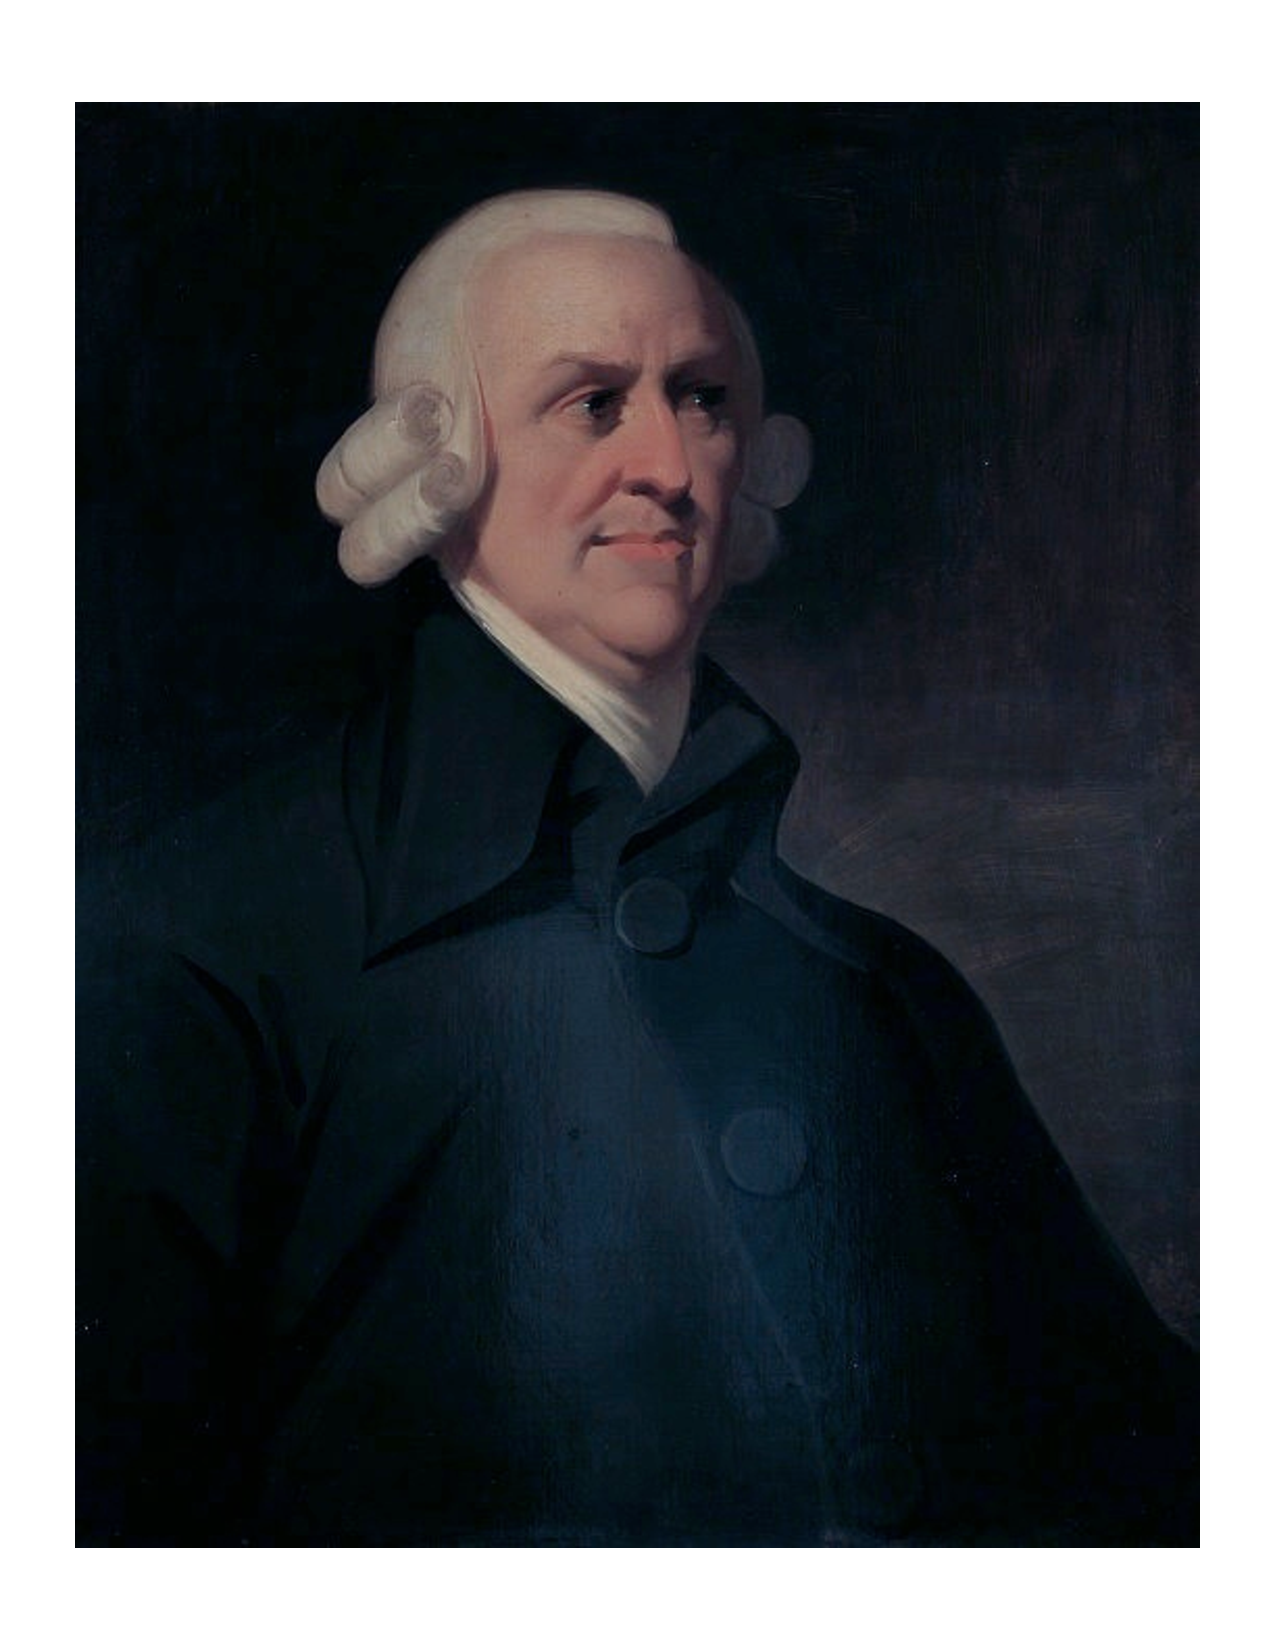
\includegraphics[width=0.35\textwidth]{figures/Adam_Smith_The_Muir_portrait}}
  \hspace{0in}
  \subfigure[Garrett Hardin: Tragedy of the Commons]{
  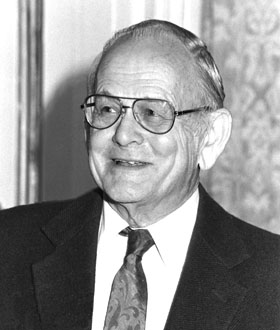
\includegraphics[width=0.35\textwidth]{figures/Garrett_Hardin.png}}
\end{figure}

\tiny{\url{http://commons.wikimedia.org/wiki/File:Adam_Smith_The_Muir_portrait.jpg}}\\
\tiny{\url{http://en.wikipedia.org/wiki/File:Garrett_Hardin.jpg}}

\note{
What can we learn about the aggregate effects of people making decisions?  Two extreme positions: Adam Smith Vs Garret Hardin.  Smith believed that people making individually selfish decisions would results in a system that is optimal for everyone.  This is a powerful statement about aggregation from individual behavior to system behavior from dogs to packs of dogs.  Hardin believe that the opposite could happen in many important cases: tragedy of the commons: imagine a bunch of shepherds around a common grazing area.  Each shepherd has incentive to add more sheep, but if everyone does the grazing area is destroyed and everyone is worse off. 

Fundamental question: to what extent do we have the wisdom of the crowds and to what extent do we have the madness of the crowd
}

\end{frame}
%%%%%%%%%%%%%%%%%%%%%%%%
\begin{frame}

\begin{itemize}
\item interdependence of decision making
\item consequences of interdependent decision making for collective outcomes
\end{itemize}

\end{frame}
%%%%%%%%%%%%%%%%%%%%%%%%
\begin{frame}

{\Large Interdependent individual decisions}

\end{frame}
%%%%%%%%%%%%%%%%%%%%%%%%%
\begin{frame}

\begin{figure}
\includegraphics[width=0.75\textwidth]{figures_book/7_1}
\end{figure}

\note{
Emphasize that all experiments are interdepent

}

\end{frame}
%%%%%%%%%%%%%%%%%%%%%%%%%
\begin{frame}

\begin{figure}
  
\includegraphics[width=.5\textwidth]{figures/asch_video.png}
\end{figure}

\url{https://www.youtube.com/watch?v=TYIh4MkcfJA}

\note{
The design is beautiful because it nicely creates two conflicting forces: evidence of the senses and social force (opinions of others).  You can imagine increasing or adjusting one or the other.

Asch experiment is a beautiful design, tunable

If you were doing a senior thesis you could do a variation of this today and it would still be interesting.  That shows the staying power of this design.
}

\end{frame}
%%%%%%%%%%%%%%%%%%%%%%%%%
\begin{frame}

\begin{figure}
  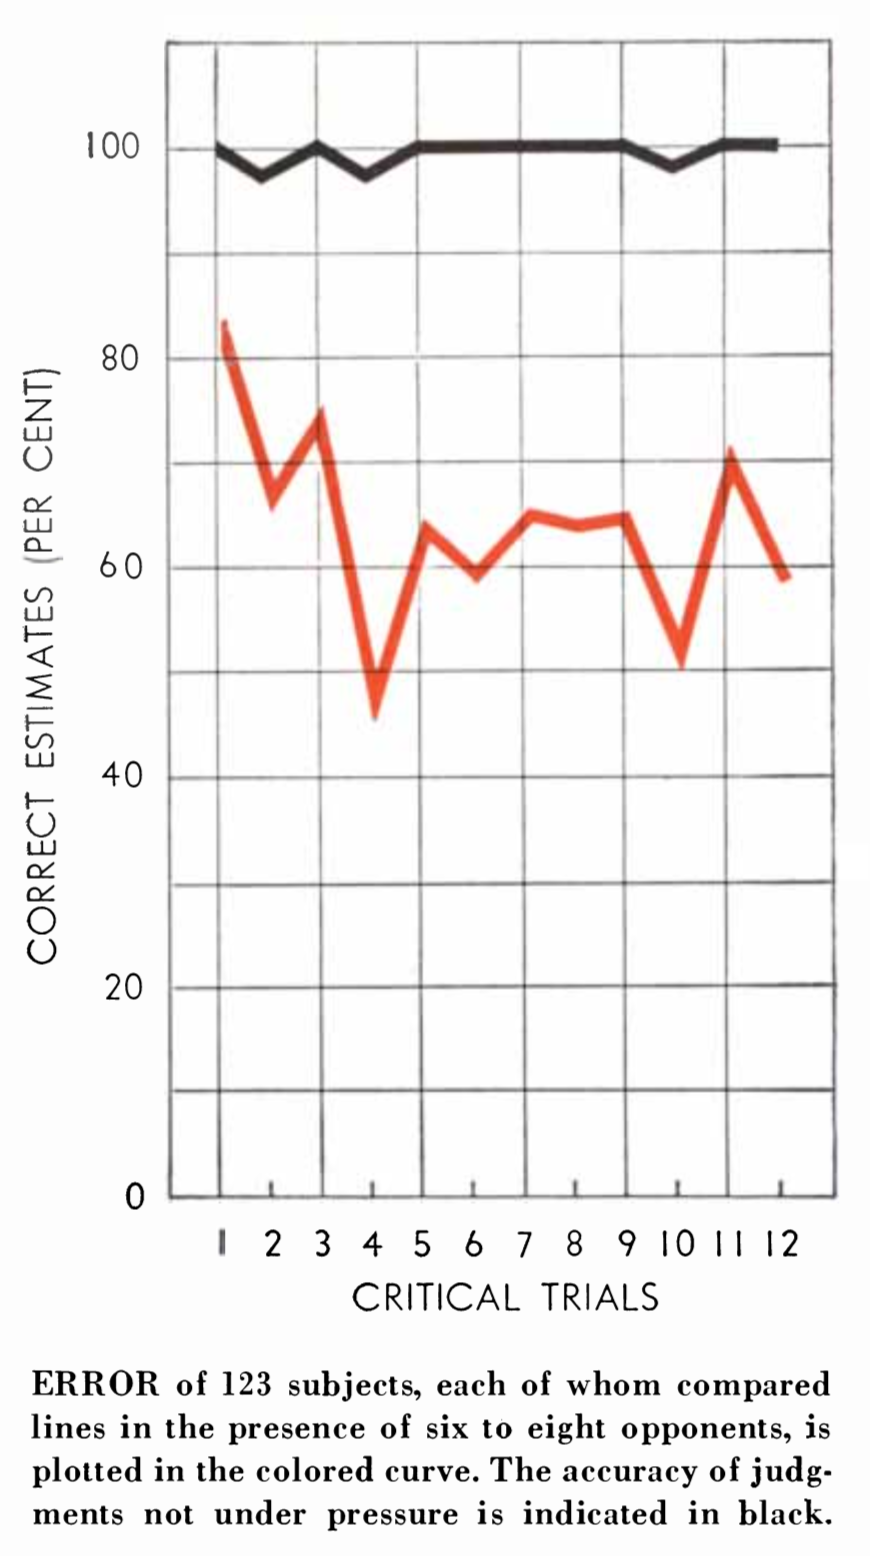
\includegraphics[width=0.35\textwidth]{figures/asch_opinions_1955_fig1.png}
\end{figure}

\note{
Errors where there are six to eight opponents and no supporters
}

\end{frame}
%%%%%%%%%%%%%%%%%%%%%%%
\begin{frame}

\begin{figure}
  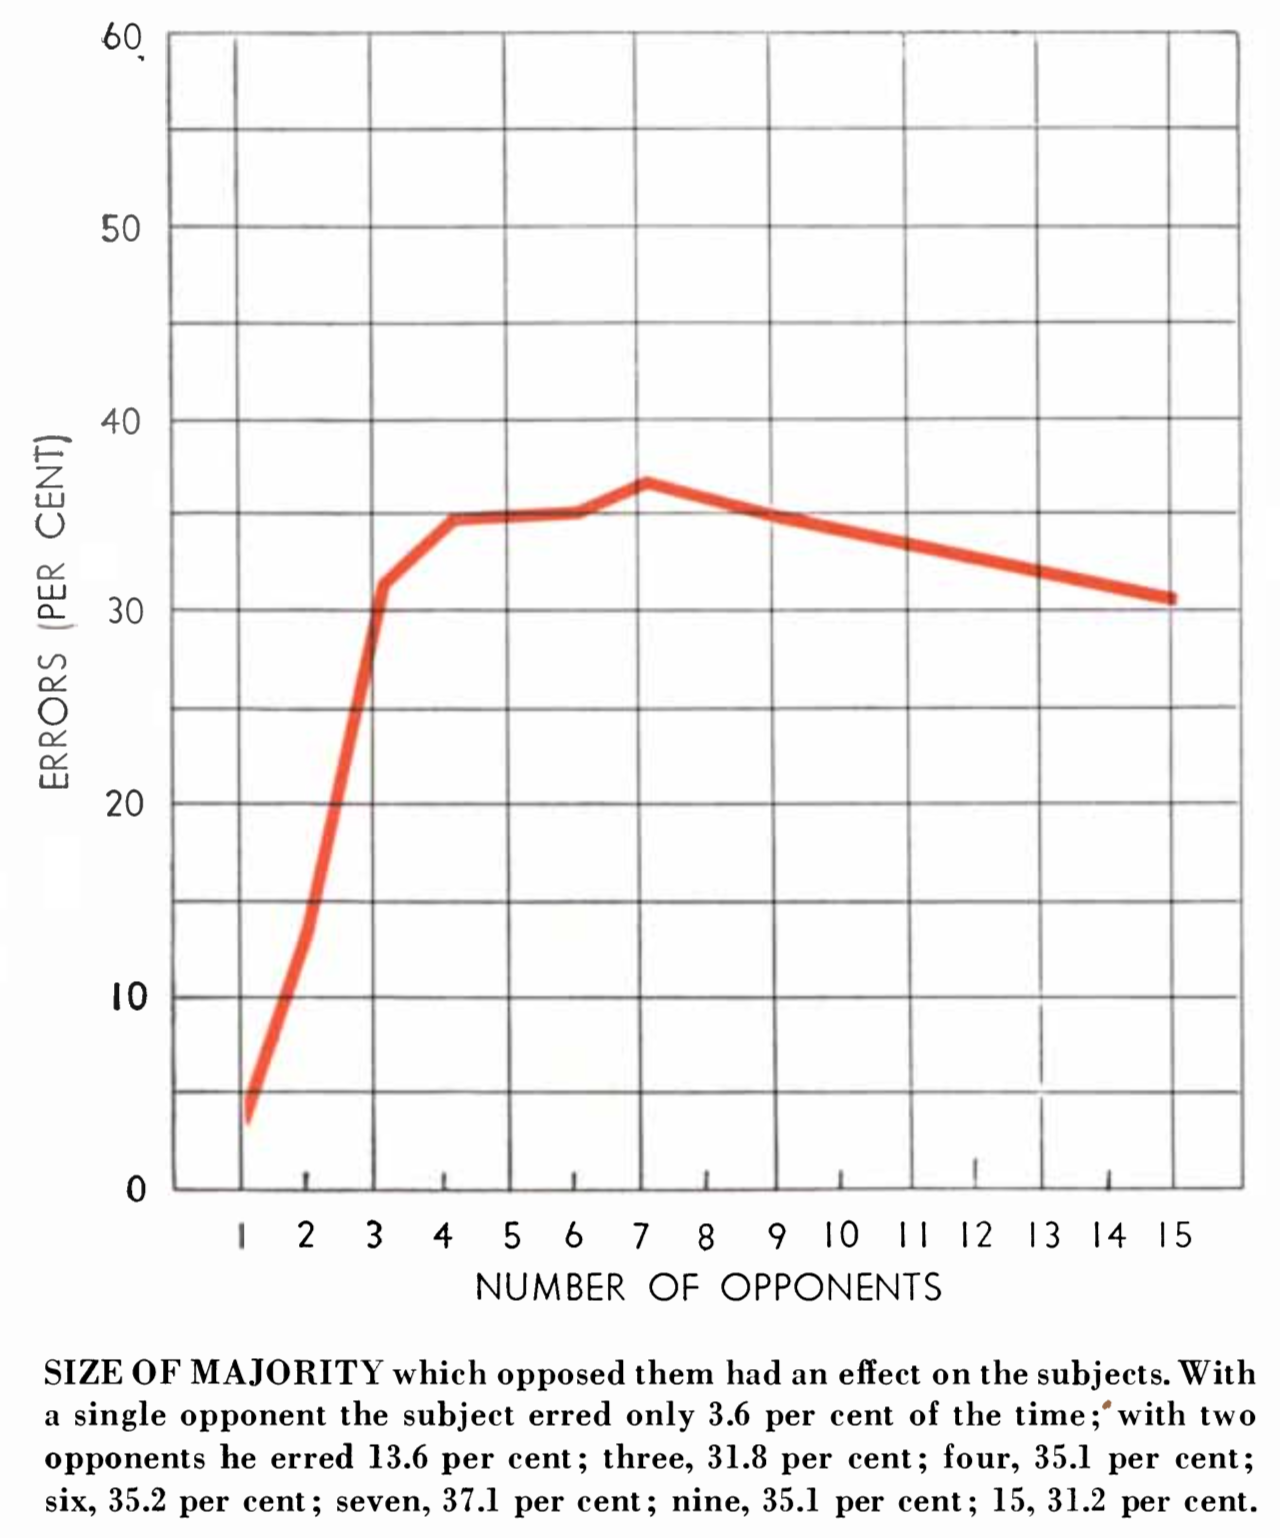
\includegraphics[width=0.35\textwidth]{figures/asch_opinions_1955_fig2.png}
 \end{figure}

\note{
Nonlinear relationship with group size.  Beyond 3 size of group does not matter.
}

\end{frame}
%%%%%%%%%%%%%%%%%%%%%%%%%
\begin{frame}

\begin{figure}
  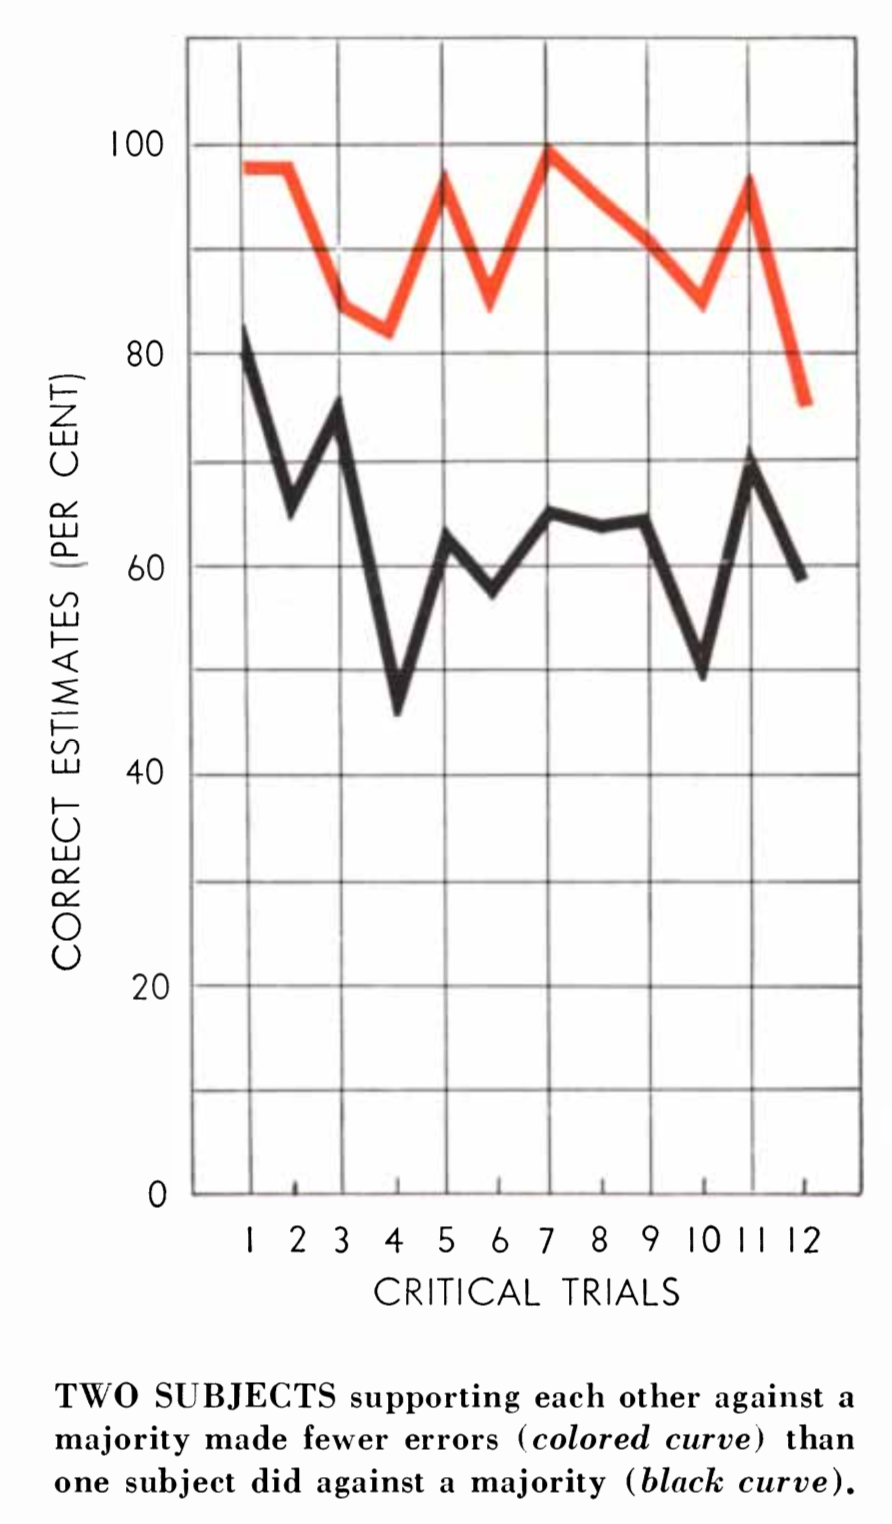
\includegraphics[width=0.35\textwidth]{figures/asch_opinions_1955_fig3.png}
 \end{figure}

\note{
Just one person being with the subject seemed to make a big difference
}

\end{frame}
%%%%%%%%%%%%%%%%%%%%%%%%%\begin{frame}
\begin{frame}

\begin{figure}

\includegraphics[height=0.90\textheight]{figures/deresieicz_excellent_2014_cover.png}
\end{figure}

\note{
Maybe you think this would never happen to you today?  Deresieicz argues that this conformity is especially prevalent at elite universities.
}

\end{frame}
%%%%%%%%%%%%%%%%%%%%%%%%%%
\begin{frame}

Which kinds of externalities where present in the Asch experiment?
\begin{enumerate}
\item information externalities
\item coercive externalities
\item market externalities
\item coordination externalities*
\end{enumerate}

\vfill
\pause
Information externalities and coercive externalities
\note{
Which were at work in the Asch experiment?  Check all that apply.

Which is at work when you try to buy an iPhone?  Hard question; it is not always easy to separate, but these forces can work as a bundle.

Note: coordination externalities are confusing.  Related to shadow of the future.

}

\end{frame}
%%%%%%%%%%%%%%%%%%%%%%%%%
\begin{frame}

What happens if we have a bunch of people who are all being influenced by each other?

\end{frame}

\end{document}
